\noindent \lecture{17}{9/12/2021}
\vspace{0.5cm}
\noindent Per semplicità ci poniamo adesso, per fare un esempio, in risonanza ($\Delta=0$).
L'hamiltoniana risulta:
\begin{equation*}
    \hat H = -\frac{A}{2}s(t) \left(I\sigma_x + Q \sigma_y \right)
\end{equation*}
Se utilizzo un segnale 'in fase' ($I=1$, $Q=0$) posso scrivere l'operatore di evoluzione temporale del nostro qubit come:
\begin{equation*}
    \hat U (t) = \exp\left[ \left(\frac{iA}{2} \int_0^t dt'\, s(t') \right) \sigma_x \right]
\end{equation*}
Se, ad esempio, scegliamo:
\begin{equation*}
    s(t') = \begin{cases} 0 \qquad \text{se $t' < 0$ o $t'> t$} \\ 1 \qquad \text{altrimenti} \end{cases}
\end{equation*}
Allora abbiamo $\hat U (t) = e^{\frac{i}{2}A t \sigma_x}$, operatore che descrive una rotazione lungo l'asse x. Dunque se stimoliamo il qubit con un segnale di questo tipo possiamo ruotare lo stato di un angolo a piacere intorno a $x$. Se procediamo nello stesso modo, ma con un segnale completamente fuori fase, otterremo in modo analogo una rotazione attorno all'asse $y$.

\subsubsection{Mixer IQ e realizzazione hardware}
Un mixer semplice (non IQ), è un componente elettronico fondamentale per la modulazione di frequenze nell'ordine del GHz. Ha 3 porte: RF, LO (\textit{local}), IF (\textit{intermediate frequency)}. LO è sempre un input, mentre le altre due porte possono essere usate alternativamente come input o output.
Supponiamo di usare RF come input e IF come output. Possiamo in questo modo fare una \textit{down conversion}: ovvero ci portiamo da alte frequenze a basse frequenze. L'output da IF sarà proporzionale al prodotto del segnale RF e del segnale LO perciò, scegliendo in modo adeguato i segnali, potremo avere una situazione del tipo:
\begin{align*}
    V_{LO} &= V_0^{LO} \cos (\omega_{LO} t) \\
    V_{RF} &= V_0^{RF} \cos (\omega_{RF} t ) \\
    V_{IF} &\propto \cos ((\omega_{LO} + \omega_{RF}) t)- \cos ((\omega_{LO} - \omega_{RF}) t)
\end{align*}
Perciò il segnale in uscita sarà diviso in due frequenze: una alta (data dalla somma delle $\omega$ che saranno quasi uguali) e una bassa (data dalla differenza fra le frequenze). Con un filtro adeguato potremo poi scegliere solo una di queste frequenze.
Per una \textit{up conversion} useremo, invece, la porta IF come input e la porta RF come output ottenendo, in modo analogo due frequenze: una data da $\omega_{LO} - \omega_{IF}$ e una data da $\omega_{LO} + \omega_{IF}$ .
Un mixer IQ è, invece, una combinazione di due diversi mixer con un totale di 4 'porte libere'. 
\begin{figure}[H]
    \centering
    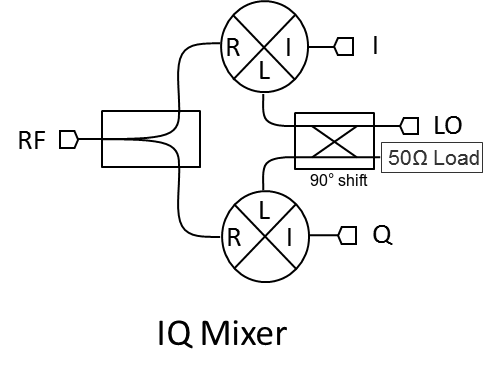
\includegraphics[width=0.6\textwidth]{images/iq_mixer.png}
\end{figure}
\noindent Supponiamo ora che I, Q e LO siano input cosinusoidali. 
A RF, dalla parte di I, arriverà un segnale $\propto \cos(\omega_{LO} + \omega_I)+ \cos (\omega_{LO} - \omega_I) $ e dalla parte di Q arriverà $\propto  \sin(\omega_{LO} + \omega_Q)+ \sin (\omega_{LO} - \omega_Q)$.
Cambiando la fase relativa fra i segnali I e Q, possiamo modulare a piacimento il segnale in uscita.

\vspace{0.5cm}

\noindent Consideriamo ora un qubit TRANSMON collegato tramite una capacità alla porta RF di un mixer IQ. Un oscillatore locale è connesso alla porta LO. Un generatore di onde a due uscite, connesso alle porte I e Q.
Con questa configurazione possiamo controllare il qubit con relativa facilità.
Assumiamo, in un primo semplice caso, che l'oscillatore sia in perfetta risonanza col qubit ($\omega_q = \omega_{LO}$). Allora, se l'output del AWG (generatore di funzioni arbitrarie) è semplicemente un segnale on/off, quando I e Q sono nulli il segnale su RF sarà anch'esso nullo (questo in realtà è vero solo in linea teorica, in realtà servirebbero minimi correttivi). Se solo I è diverso da zero otterremo un segnale totalmente fuori fase rispetto a LO, mentre se solo Q è diverso da zero il segnale sarà totalmente in fase.
Se, invece, il segnale di AWG ha frequenza $\omega_{AWG}$ e usiamo un oscillatore con frequenza $\omega_{LO}=\omega_q - \omega_{AWG}$, possiamo usare I e Q in modo da avere a piacimento un segnale in fase o fuori fase. Così facendo otterremo sempre due frequenze, di cui solo una utile al controllo. Ciò che viene fatto usualmente è di sfasare il segnale in ingresso di I e Q di 90°, in modo che il segnale in uscita RF abbia un'unica frequenza caratteristica (si parla di \textit{Single Sideband modulation - SSB}).
\begin{figure}[H]
    \centering
    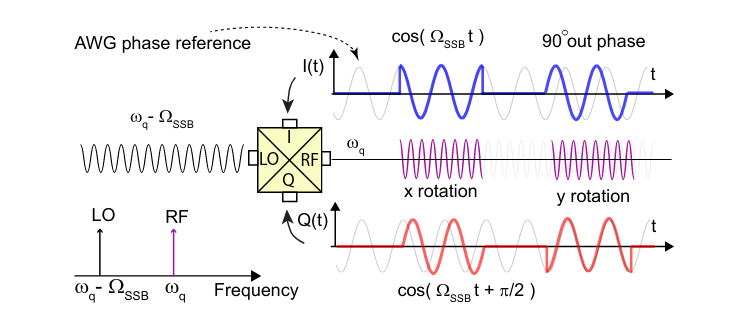
\includegraphics[width= \textwidth]{images/single_sideband_modulation.png}
    \caption{Single Sideband Modulation (SSB): By up-converting the LO signal by $\Omega_{SSB}$ the mixer
outputs at qubit frequency. The relative phase of SSB pulses determines the phase of the output signal thus
the direction of the rotation for the qubit. \url{https://arxiv.org/pdf/1904.09291.pdf}}
\end{figure}
\noindent In questo modo possiamo a piacimento ruotare lo stato del qubit intorno agli assi x-y coi meccanismi di controllo XY che abbiamo già illustrato.
Nel caso avessimo più qubit tutti collegati al medesima linea (connessa a RF) possiamo variare la frequenza $\omega_{AWG}$ in modo da stimolare in risonanza solo un qubit alla volta. Questo chiaramente a patto che i qubit abbiano frequenze caratteristiche diverse (proprietà facilmente ottenibile con un qubit TRANSMON simmetrico e una corretta modulazione del flusso interno al circuito).

\section{Misurazioni e circuit QED}

Per la misurazione di un qubit, considereremo un TRANSMON. Utilizzeremo la teoria QED per circuiti (\textit{circuit QED}) che è un'estensione della \textit{cavity QED}. Quest'ultima teoria considera una cavità RF dove, essendoci delle proprietà di risonanza, possono stabilirsi delle onde stazionarie (dei modi di oscillazione che corrispondono a fotoni a frequenze diverse). 
La cosa interessante è che posso partire da una cavità "vuota" (in un qualche \textit{ground state} $\ket 0$) ed eccitare il sistema a $\ket 1$ o $\ket 2$ stimolando la cavità con l'appropriata onda.
Se posso limitarmi ai primi due stati ho, in principio, un qubit.

\subsection{Cavity QED}
\subsubsection{Misurazione di una cavità con un atomo di Rydberg}
Per misurare il suo stato posso far attraversare la cavità da un atomo con frequenza di transizione (una cavità è un oscillatore armonico quantistico) uguale a quella caratteristica della cavità/qubit (che posso modulare). L'atomo entra in interazione col qubit tramite oscillazioni del suo stato simili a quelle di Rabi perciò, scegliendo con cautela velocità dell'atomo e dimensioni della cavità, posso far sì che l'atomo subisca una rotazione di $\pi$ mentre la cavità non ruoti (dunque abbiamo una QND).
Negli esperimenti che portarono all'assegnazione del premio Nobel per la fisica del 2012 \footnote{\url{https://www.nobelprize.org/uploads/2018/06/advanced-physicsprize2012.pdf}}, venivano usati atomi di rubidio (Rb) (utili perché dotati di grande dipolo elettrico) sfruttando la cosiddetta interferometria Ramsey. La configurazione hardware dell'esperimento comprendeva, in particolare, due segnali RF che l'atomo attraversava prima (R1) e dopo (R2) attraverso il qubit atti alla misurazione e al controllo dello stato atomico (tramite tecnologie più classiche).
Dell'atomo vengono usati, in particolare, 3 stati: $\ket i$, $\ket g$ e $\ket e$ (dati da livelli di Rydberg in approssimazione di atomo sferico). Dove la differenza di energia fra $\ket g$ e $\ket e$ corrisponde alla frequenza di risonanza del qubit.
Assumiamo che l'atomo sia inizialmente nello stato $\ket g$ e che vogliamo misurare se la cavità si trova nello stato $\ket 0$ o $\ket 1$. Lo inviamo attraverso la cavità R1 (che ha frequenza caratteristica data dalla differenza di energia fra $\ket g$ e $\ket i$) e gli diamo un impulso di $\pi/2$. L'atomo, dopo R1, si troverà quindi in uno stato: $\frac{1}{\sqrt 2} \left( \ket g + \ket i \right)$. 
A questo punto l'atomo attraversa la cavità principale interagendo col campo elettrostatico quantizzato tramite il proprio dipolo elettrico. A seconda dello stato della cavità, l'accoppiamento fra campo elettrico e dipolo opererà in modo differente. L'hamiltoniana di interazione fra atomo e cavità viene detta hamiltoniana di Jaynes-Cumming e avrà chiaramente degli autostati che dipendono dagli stati del campo e dell'atomo. Essendoci una sovrapposizione di stati, avremo anche una precessione data dalla differenza di energia degli autostati ovvero avremo oscillazioni di Rabi. Progettando in modo adeguato l'esperimento, posso far sì che la cavità mi dia un impulso $\pi$. L'evoluzione dello stato è data da:
\begin{equation*}
    \cos \left( \frac{\Omega t}{2}\right) \ket{g, 1}+ \sin \left( \frac{\Omega t}{2}\right) \ket{e, 0}
\end{equation*}
L'atomo, dunque, varierà stato solo se la cavità è in $\ket 1$ e arriverà a $\frac{1}{\sqrt{2}}\left( -\ket g + \ket i \right)$ (ho $\Omega t/2=2\pi$).
Attraversando poi R2 (anch'essa $\pi/2$ come R1) lo stato andrà in $\ket g$ o $\ket e$ (a seconda del segno relativo fra $\ket i$ e $\ket g$).